\documentclass[letterpaper,11pt]{article}

% -------------------------
% PAQUETES
% -------------------------
\usepackage[spanish]{babel}
\usepackage[utf8]{inputenc}
\usepackage[T1]{fontenc}
\usepackage{graphicx}
\usepackage{geometry}
\usepackage{array}
\usepackage{setspace}
\usepackage{titlesec}
\usepackage{enumitem}
\geometry{margin=2.5cm}
\usepackage{amsmath}

\usepackage{float}
\usepackage{xcolor}
\usepackage{realboxes}
\definecolor{lightgrey}{rgb}{0.95,0.95,0.95} % El color del fondo

% Creamos un comando personalizado llamado \code
\newcommand{\code}[1]{\Colorbox{lightgrey}{\texttt{#1}}}

% -------------------------
% INICIO DOCUMENTO
% -------------------------

\begin{document}

\noindent
\begin{minipage}{0.40\textwidth}
    
\includegraphics[width=\linewidth]{logoUSM.png}
\end{minipage}
\hfill
\begin{minipage}{0.60\textwidth}
    \raggedleft
    \textbf{INGENIERÍA COMERCIAL}\\
    \textbf{2026-2}
\end{minipage}

\vspace{0.4cm}
\hrule
\vspace{0.1cm}

% -------------------------
% INFORMACIÓN CURSO
% -------------------------
\begin{center}
        {\Large \textbf{Control 1}}\\
    Econometría ICS-294\\
    II Semestre 2026\\
    \vspace{0.3cm}
    Profesor: Francisco Alfaro Medina \\

\end{center}



\textbf{Instrucciones:} 

\begin{itemize}
    \item El trabajo deberá entregarse resuelto a mano.
    \item Cuide la presentación y la redacción de sus respuestas.
\end{itemize}

\section{Preguntas}



 
\begin{enumerate}



\item Sean $\overline{X}_n$ y $S_n^2$ el promedio y la varianza para la muestra $X_1, \ldots, X_n$ y sean $\overline{X}_{n+1}$ y $S_{n+1}^2$ estas cantidades cuando se añade a la muestra una observación adicional $X_{n+1}$.
    \begin{enumerate}
        \item[(a)] Demuestre cómo se puede calcular $\overline{X}_{n+1}$ a partir de $\overline{X}_n$ y $X_{n+1}$.
        \item[(b)] Demuestre que
        \[
        S_{n+1}^2 = \frac{n}{n+1} \left\{ S_n^2 + \frac{1}{n+1} \left( X_{n+1} - \overline{X}_n \right)^2 \right\}.
        \]
    \end{enumerate}

\textbf{Desarrollo}

\textbf{(a)} Por definición del promedio muestral:
\[
\overline{X}_{n+1}
= \frac{1}{n+1}\sum_{i=1}^{n+1}X_i
= \frac{1}{n+1}\left(\sum_{i=1}^{n}X_i + X_{n+1}\right).
\]
Como $\sum_{i=1}^{n}X_i=n\overline{X}_n$, se obtiene
\[
\boxed{\overline{X}_{n+1}=\frac{n\overline{X}_n+X_{n+1}}{n+1}.}
\]

\textbf{(b)} Usando la definición $S_n^2=\frac{1}{n}\sum_{i=1}^n X_i^2-\overline{X}_n^2$, tenemos
\begin{align*}
S_{n+1}^2
&= \frac{1}{n+1}\sum_{i=1}^{n+1}X_i^2-\overline{X}_{n+1}^2\\
&= \frac{1}{n+1}\left(\sum_{i=1}^{n}X_i^2+X_{n+1}^2\right)
-\frac{1}{(n+1)^2}\left(n\overline{X}_n+X_{n+1}\right)^2\\
&= \frac{1}{n+1}\left(nS_n^2+n\overline{X}_n^2+X_{n+1}^2\right)
-\frac{1}{(n+1)^2}\left(n^2\overline{X}_n^2+2n\overline{X}_nX_{n+1}+X_{n+1}^2\right)\\
&= \frac{n}{n+1}S_n^2
+\frac{n}{(n+1)^2}\left(\overline{X}_n^2-2\overline{X}_nX_{n+1}+X_{n+1}^2\right)\\
&= \frac{n}{n+1}S_n^2+\frac{n}{(n+1)^2}\left(X_{n+1}-\overline{X}_n\right)^2.
\end{align*}
Por lo tanto,
\[
\boxed{
S_{n+1}^2 = \frac{n}{n+1} \left\{ S_n^2 + \frac{1}{n+1} \left( X_{n+1} - \overline{X}_n \right)^2 \right\}.
}
\]



\item Una empresa de tecnología quiere estimar el tiempo promedio (en minutos) que sus usuarios pasan diariamente en su aplicación móvil. Para ello, selecciona una muestra aleatoria de 150 usuarios y obtiene un tiempo promedio de 42 minutos, con una desviación estándar poblacional conocida de 12 minutos.

Construya un intervalo de confianza del 95\% para el tiempo promedio diario que los usuarios pasan en la aplicación.

\textbf{Desarrollo}

Como la desviación estándar poblacional es conocida, usamos
\[
\bar{x}\pm z_{\alpha/2}\frac{\sigma}{\sqrt{n}}.
\]
Con $\bar{x}=42$, $\sigma=12$, $n=150$ y $z_{0,025}=1,96$:
\[
42\pm 1,96\frac{12}{\sqrt{150}}
=42\pm 1,92.
\]
Así, el intervalo de confianza al 95\% es
\[
\boxed{[40,08,\;43,92].}
\]
Con 95\% de confianza, el tiempo promedio diario se encuentra entre 40,08 y 43,92 minutos.

\item Un partido político desea estimar la proporción de votantes que apoyan una nueva reforma tributaria. En una encuesta aplicada a 500 votantes seleccionados aleatoriamente, 215 declararon estar a favor de la reforma.

Construya un intervalo de confianza del 95\% para la proporción de votantes que apoyan la reforma tributaria.

\textbf{Desarrollo}

La proporción muestral es
\[
\hat{p}=\frac{215}{500}=0,43.
\]
El intervalo de confianza al 95\% para una proporción es
\[
\hat{p}\pm z_{\alpha/2}\sqrt{\frac{\hat{p}(1-\hat{p})}{n}}.
\]
Luego,
\[
0,43\pm 1,96\sqrt{\frac{0,43(1-0,43)}{500}}
=0,43\pm 0,0434.
\]
Por lo tanto,
\[
\boxed{[0,3866,\;0,4734].}
\]
Con 95\% de confianza, la proporción de votantes que apoya la reforma está entre 38,66\% y 47,34\%.

\item En un hospital se realiza un estudio sobre las diferencias en el peso de los bebés al nacer entre dos grupos de mujeres embarazadas: aquellas que viven en el campo y aquellas que viven en la ciudad. Los datos recabados se resumen en la siguiente tabla:
\begin{center}
    \begin{tabular}{| l| c | c| c|}
\hline
& Tamaño muestra& Peso medio muestra & Desviación estándar poblacional \\ \hline
Campo &240 &3,8&0,6 \\
Ciudad & 300& 3,5& 0,8\\ \hline
\end{tabular}
\end{center}
Determine si el promedio del peso al nacer de los bebés difiere dependiendo si sus madres viven en la ciudad o en el campo con 95\% de confianza.

\textbf{Desarrollo}

Queremos analizar la diferencia de medias $\mu_{campo}-\mu_{ciudad}$. La diferencia muestral es
\[
\bar{X}_{campo}-\bar{X}_{ciudad}=3,8-3,5=0,3.
\]
El error estándar es
\[
\sqrt{\frac{0,6^2}{240}+\frac{0,8^2}{300}}
=\sqrt{0,0015+0,00213}
=0,0603.
\]
El intervalo de confianza al 95\% es
\[
0,3\pm 1,96(0,0603)
=0,3\pm 0,1182.
\]
Por lo tanto,
\[
\boxed{[0,1818,\;0,4182].}
\]
Como el intervalo no contiene al cero, existe evidencia al 95\% de confianza para concluir que el peso promedio al nacer difiere entre ambos grupos. Además, como el intervalo es positivo, el peso promedio de los bebés cuyas madres viven en el campo es mayor que el de los bebés cuyas madres viven en la ciudad.

\item ¿En qué consiste el método de Mínimos Cuadrados Ordinarios (MCO)?

\textbf{Respuesta}

El método de Mínimos Cuadrados Ordinarios consiste en estimar los parámetros de una regresión eligiendo la recta que minimiza la suma de los residuos al cuadrado. En el modelo lineal simple,
\[
Y_i=\beta_0+\beta_1X_i+u_i,
\]
MCO escoge $\hat{\beta}_0$ y $\hat{\beta}_1$ para minimizar
\[
\sum_{i=1}^{n}\hat{u}_i^2
=\sum_{i=1}^{n}(Y_i-\hat{\beta}_0-\hat{\beta}_1X_i)^2.
\]
La idea es encontrar la recta que, en promedio, queda lo más cerca posible de los datos observados, penalizando más los errores grandes debido al cuadrado.


\item ¿Cuáles son los supuestos claves del método MCO (explique) y qué sucede si se violan?

\textbf{Respuesta}

Los supuestos claves de MCO son:
\begin{itemize}
    \item \textbf{Linealidad en los parámetros:} el modelo debe poder escribirse como una relación lineal en los coeficientes. Si se especifica mal la forma funcional, los estimadores pueden estar sesgados.
    \item \textbf{Muestra aleatoria:} las observaciones deben provenir de un proceso de muestreo aleatorio. Si no se cumple, puede haber sesgo de selección y los resultados no serán representativos.
    \item \textbf{Variabilidad en la variable explicativa:} $X$ debe variar entre observaciones. Si $X$ no varía, no se puede estimar su efecto sobre $Y$.
    \item \textbf{Exogeneidad o media condicional cero:} se requiere que $E(u_i|X_i)=0$. Si se viola, por ejemplo por variables omitidas, simultaneidad o error de medición, los estimadores MCO son sesgados e inconsistentes.
    \item \textbf{No multicolinealidad perfecta:} en modelos con varias variables explicativas, ninguna variable debe ser combinación lineal exacta de otra. Si existe multicolinealidad perfecta, no se pueden estimar los coeficientes.
    \item \textbf{Homocedasticidad:} la varianza del error debe ser constante condicional en las variables explicativas. Si hay heterocedasticidad, los estimadores pueden seguir siendo insesgados bajo exogeneidad, pero los errores estándar usuales son incorrectos.
    \item \textbf{No autocorrelación:} los errores no deben estar correlacionados entre observaciones. Si se viola, especialmente en series de tiempo, los errores estándar y las pruebas de hipótesis pueden ser inválidos.
\end{itemize}
En resumen, las violaciones más graves son aquellas que afectan la exogeneidad, porque generan sesgo e inconsistencia. Otras, como heterocedasticidad o autocorrelación, afectan principalmente la inferencia si no se corrigen los errores estándar.

\item Un investigador estudia el efecto de las horas de sueño sobre el rendimiento académico. Se tienen datos de 5 estudiantes:
\begin{center}
    \begin{tabular}{| c | c | c |}
\hline
\textbf{Estudiante} & \textbf{Horas de sueño ($X$)} & \textbf{Nota ($Y$)} \\ \hline
1 & 5 & 3,5 \\
2 & 6 & 4,0 \\
3 & 7 & 5,0 \\
4 & 8 & 5,5 \\
5 & 9 & 6,0 \\ \hline
\end{tabular}
\end{center}
\begin{enumerate}[label=(\alph*)]
    \item Calcule los estimadores MCO $\hat{\beta}_0$ y $\hat{\beta}_1$ e interprete económicamente cada uno.
    \item Calcule los valores ajustados $\hat{y}_i$ y los residuos $\hat{u}_i$. Verifique que $\sum \hat{u}_i = 0$.
    \item Calcule SST, SSE, SSR y el coeficiente $R^2$. Interprete.
\end{enumerate}

\textbf{Desarrollo}

Primero calculamos los promedios:
\[
\bar{X}=\frac{5+6+7+8+9}{5}=7,
\qquad
\bar{Y}=\frac{3,5+4,0+5,0+5,5+6,0}{5}=4,8.
\]

\textbf{(a)} La pendiente MCO es
\[
\hat{\beta}_1=
\frac{\sum (X_i-\bar{X})(Y_i-\bar{Y})}{\sum (X_i-\bar{X})^2}.
\]
Calculando:
\[
\sum (X_i-\bar{X})(Y_i-\bar{Y})=6,5,
\qquad
\sum (X_i-\bar{X})^2=10.
\]
Por lo tanto,
\[
\hat{\beta}_1=\frac{6,5}{10}=0,65.
\]
El intercepto es
\[
\hat{\beta}_0=\bar{Y}-\hat{\beta}_1\bar{X}=4,8-0,65(7)=0,25.
\]
La recta estimada es
\[
\boxed{\hat{Y}_i=0,25+0,65X_i.}
\]
Interpretación: por cada hora adicional de sueño, la nota esperada aumenta en 0,65 puntos. El intercepto indica que, si un estudiante durmiera 0 horas, la nota predicha sería 0,25; en este contexto su interpretación económica es limitada, porque 0 horas está fuera del rango observado.

\textbf{(b)} Los valores ajustados y residuos son:
\begin{center}
\begin{tabular}{|c|c|c|c|c|}
\hline
Estudiante & $X_i$ & $Y_i$ & $\hat{Y}_i=0,25+0,65X_i$ & $\hat{u}_i=Y_i-\hat{Y}_i$ \\ \hline
1 & 5 & 3,5 & 3,5 & 0,0 \\
2 & 6 & 4,0 & 4,15 & -0,15 \\
3 & 7 & 5,0 & 4,8 & 0,20 \\
4 & 8 & 5,5 & 5,45 & 0,05 \\
5 & 9 & 6,0 & 6,10 & -0,10 \\ \hline
\end{tabular}
\end{center}
Se verifica que
\[
\sum \hat{u}_i=0-0,15+0,20+0,05-0,10=0.
\]

\textbf{(c)} La suma total de cuadrados es
\[
SST=\sum (Y_i-\bar{Y})^2=4,3.
\]
La suma explicada por la regresión es
\[
SSE=\sum(\hat{Y}_i-\bar{Y})^2=4,225.
\]
La suma de residuos al cuadrado es
\[
SSR=\sum \hat{u}_i^2=0,075.
\]
Dependiendo de la convención usada, algunas clases llaman $SSE$ a la suma de errores y $SSR$ a la suma explicada. En esta pauta se reportan ambas cantidades claramente: suma explicada $=4,225$ y suma residual $=0,075$.

El coeficiente de determinación es
\[
R^2=\frac{\sum(\hat{Y}_i-\bar{Y})^2}{\sum(Y_i-\bar{Y})^2}
=\frac{4,225}{4,3}=0,9826.
\]
Equivalentemente, usando $R^2=1-\frac{\sum\hat{u}_i^2}{SST}$:
\[
R^2=1-\frac{0,075}{4,3}=0,9826.
\]
\[
\boxed{R^2\approx 0,983.}
\]
Esto significa que aproximadamente el 98,3\% de la variabilidad de las notas se explica por las horas de sueño en esta muestra.

\item Dada una muestra bivariada $(X_1, Y_1), \ldots, (X_n, Y_n)$, considere el modelo de regresión lineal simple $Y_i = \beta_0 + \beta_1 X_i + \epsilon_i$. Suponga que deseamos encontrar el intercepto y la pendiente que minimizan el error cuadrático, sujeto a la restricción de que la recta debe pasar por el punto $(a,b)$, donde $a$ y $b$ son números reales conocidos. Muestre que la solución de este problema, denotada por $(\widehat{\beta}_0, \widehat{\beta}_1)$, está dada por
\[
\begin{cases}
    \widehat{\beta}_0 = b - \widehat{\beta}_1 a \\[6pt]
    \widehat{\beta}_1 = \dfrac{\sum_{i=1}^{n} (Y_i - b)(X_i - a)}{\sum_{i=1}^{n} (X_i - a)^2}
\end{cases}.
\]

\textbf{Desarrollo}

Si la recta debe pasar por el punto $(a,b)$, entonces debe cumplirse
\[
b=\beta_0+\beta_1a.
\]
Por lo tanto,
\[
\beta_0=b-\beta_1a.
\]
Sustituyendo esta restricción en el modelo, la recta queda:
\[
\hat{Y}_i=b-\beta_1a+\beta_1X_i
=b+\beta_1(X_i-a).
\]
Entonces el problema consiste en minimizar, respecto de $\beta_1$,
\[
g(\beta_1)=\sum_{i=1}^{n}\left[Y_i-b-\beta_1(X_i-a)\right]^2.
\]
Derivando e igualando a cero:
\[
g'(\widehat{\beta}_1)
=-2\sum_{i=1}^{n}\left[Y_i-b-\widehat{\beta}_1(X_i-a)\right](X_i-a)=0.
\]
Dividiendo por $-2$:
\[
\sum_{i=1}^{n}\left[Y_i-b-\widehat{\beta}_1(X_i-a)\right](X_i-a)=0.
\]
Distribuyendo:
\[
\sum_{i=1}^{n}(Y_i-b)(X_i-a)
-\widehat{\beta}_1\sum_{i=1}^{n}(X_i-a)^2=0.
\]
Despejando $\widehat{\beta}_1$:
\[
\widehat{\beta}_1\sum_{i=1}^{n}(X_i-a)^2
=\sum_{i=1}^{n}(Y_i-b)(X_i-a).
\]
Si $\sum_{i=1}^{n}(X_i-a)^2>0$, se obtiene
\[
\boxed{
\widehat{\beta}_1=
\frac{\sum_{i=1}^{n}(Y_i-b)(X_i-a)}
{\sum_{i=1}^{n}(X_i-a)^2}.
}
\]
Finalmente,
\[
\boxed{\widehat{\beta}_0=b-\widehat{\beta}_1a.}
\]
Además,
\[
g''(\beta_1)=2\sum_{i=1}^{n}(X_i-a)^2>0,
\]
por lo que la solución corresponde a un mínimo.

\item En el estudio de Miguel y Kremer (2004) sobre el programa de desparasitación escolar en Kenia.
   


\begin{enumerate}
    \item Describa brevemente cómo se asignaron las escuelas al tratamiento y qué tipo de aleatorización se utilizó. Explique por qué se eligió aleatorizar a nivel de escuela y no a nivel de individuo.

    \item  ¿Cuáles son las \textbf{externalidades} a las que se hace referencia en este contexto? 
	 ¿Qué ventajas presenta este diseño de muestreo y tratamiento para identificar tanto los efectos directos como las externalidades del programa?
\end{enumerate}

\textbf{Respuesta}

\begin{enumerate}
    \item Las escuelas fueron asignadas al programa de manera aleatoria, pero la aleatorización se realizó a nivel de escuela, no a nivel de estudiante. Es decir, algunas escuelas recibieron el tratamiento antes que otras, permitiendo comparar escuelas tratadas y no tratadas.
    
    Se eligió aleatorizar a nivel de escuela porque el tratamiento podía generar efectos indirectos sobre otros niños. Si se hubiera tratado solo a algunos estudiantes dentro de una misma escuela, los estudiantes no tratados también podrían haberse beneficiado por una menor transmisión de parásitos. Esto habría contaminado la comparación entre tratados y controles dentro de la misma escuela.
    
    \item Las externalidades corresponden a los beneficios indirectos que reciben personas que no fueron tratadas directamente. En este caso, al desparasitar a un grupo de estudiantes, disminuye la carga parasitaria y la transmisión dentro de la escuela y también en zonas cercanas. Por ello, estudiantes no tratados o estudiantes de escuelas cercanas pueden mejorar su salud y asistencia escolar aun sin recibir directamente el medicamento.
    
    La ventaja del diseño es que permite estimar tanto el efecto directo del tratamiento sobre las escuelas tratadas como los efectos indirectos sobre escuelas cercanas o grupos no tratados. Al asignar el tratamiento por escuelas y considerar la ubicación geográfica, el estudio puede distinguir entre el impacto del programa en quienes lo reciben y las externalidades generadas por menor contagio en el entorno.
\end{enumerate}

\end{enumerate}


\newpage
\section{Formulario}
\begin{itemize}
\item El intervalo de confianza de $100(1-\alpha)\%$ para la media poblacional $\mu$ con $\sigma$  \emph{\textbf{conocido}} es:
$\color{red}{\bar{x} \pm z_{\frac{\alpha}{2}}\frac{\sigma}{\sqrt{n}}}$
\item El intervalo de confianza de $100(1-\alpha)\%$ para la diferencia de medias
$\mu_x-\mu_y$ es  con $\sigma_x$ y $\sigma_y$   \emph{\textbf{conocidos}} es:
${\color{red}(\bar{X}-\bar{Y}) \pm z_{\frac{\alpha}{2}}\sqrt{\frac{\sigma_x^2}{n_x}+\frac{\sigma_y^2}{n_y}}}$
\item El intervalo de confianza de $100(1-\alpha)\%$ para la proporción poblacional $p$ es:
${\color{red}\hat{p} \pm z_{\frac{\alpha}{2}}\sqrt{\dfrac{\hat{p}(1-\hat{p})}{n}}}$
\end{itemize}

\begin{figure}[H]
    \centering
    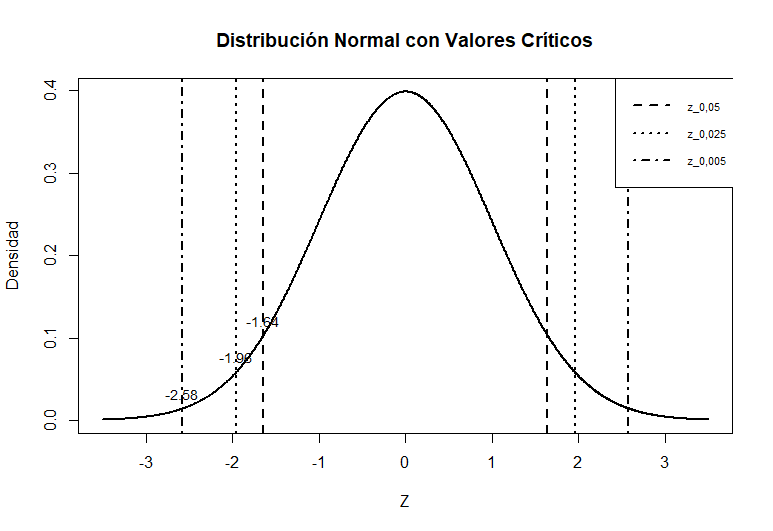
\includegraphics[width=0.9\linewidth]{normal_critic.png}
\end{figure}
 

\end{document}
